\documentclass[twoside]{book}

% Packages required by doxygen
\usepackage{calc}
\usepackage{doxygen}
\usepackage{graphicx}
\usepackage[utf8]{inputenc}
\usepackage{makeidx}
\usepackage{multicol}
\usepackage{multirow}
\usepackage{textcomp}
\usepackage[table]{xcolor}

% Font selection
\usepackage[T1]{fontenc}
\usepackage{mathptmx}
\usepackage[scaled=.90]{helvet}
\usepackage{courier}
\usepackage{amssymb}
\usepackage{sectsty}
\renewcommand{\familydefault}{\sfdefault}
\allsectionsfont{%
  \fontseries{bc}\selectfont%
  \color{darkgray}%
}
\renewcommand{\DoxyLabelFont}{%
  \fontseries{bc}\selectfont%
  \color{darkgray}%
}

% Page & text layout
\usepackage{geometry}
\geometry{%
  a4paper,%
  top=2.5cm,%
  bottom=2.5cm,%
  left=2.5cm,%
  right=2.5cm%
}
\tolerance=750
\hfuzz=15pt
\hbadness=750
\setlength{\emergencystretch}{15pt}
\setlength{\parindent}{0cm}
\setlength{\parskip}{0.2cm}
\makeatletter
\renewcommand{\paragraph}{%
  \@startsection{paragraph}{4}{0ex}{-1.0ex}{1.0ex}{%
    \normalfont\normalsize\bfseries\SS@parafont%
  }%
}
\renewcommand{\subparagraph}{%
  \@startsection{subparagraph}{5}{0ex}{-1.0ex}{1.0ex}{%
    \normalfont\normalsize\bfseries\SS@subparafont%
  }%
}
\makeatother

% Headers & footers
\usepackage{fancyhdr}
\pagestyle{fancyplain}
\fancyhead[LE]{\fancyplain{}{\bfseries\thepage}}
\fancyhead[CE]{\fancyplain{}{}}
\fancyhead[RE]{\fancyplain{}{\bfseries\leftmark}}
\fancyhead[LO]{\fancyplain{}{\bfseries\rightmark}}
\fancyhead[CO]{\fancyplain{}{}}
\fancyhead[RO]{\fancyplain{}{\bfseries\thepage}}
\fancyfoot[LE]{\fancyplain{}{}}
\fancyfoot[CE]{\fancyplain{}{}}
\fancyfoot[RE]{\fancyplain{}{\bfseries\scriptsize Generated on Fri Sep 5 2014 01\-:25\-:50 for Image\-R\-M\-I by Doxygen }}
\fancyfoot[LO]{\fancyplain{}{\bfseries\scriptsize Generated on Fri Sep 5 2014 01\-:25\-:50 for Image\-R\-M\-I by Doxygen }}
\fancyfoot[CO]{\fancyplain{}{}}
\fancyfoot[RO]{\fancyplain{}{}}
\renewcommand{\footrulewidth}{0.4pt}
\renewcommand{\chaptermark}[1]{%
  \markboth{#1}{}%
}
\renewcommand{\sectionmark}[1]{%
  \markright{\thesection\ #1}%
}

% Indices & bibliography
\usepackage{natbib}
\usepackage[titles]{tocloft}
\setcounter{tocdepth}{3}
\setcounter{secnumdepth}{5}
\makeindex

% Hyperlinks (required, but should be loaded last)
\usepackage{ifpdf}
\ifpdf
  \usepackage[pdftex,pagebackref=true]{hyperref}
\else
  \usepackage[ps2pdf,pagebackref=true]{hyperref}
\fi
\hypersetup{%
  colorlinks=true,%
  linkcolor=blue,%
  citecolor=blue,%
  unicode%
}

% Custom commands
\newcommand{\clearemptydoublepage}{%
  \newpage{\pagestyle{empty}\cleardoublepage}%
}


%===== C O N T E N T S =====

\begin{document}

% Titlepage & ToC
\hypersetup{pageanchor=false}
\pagenumbering{roman}
\begin{titlepage}
\vspace*{7cm}
\begin{center}%
{\Large Image\-R\-M\-I }\\
\vspace*{1cm}
{\large Generated by Doxygen 1.8.6}\\
\vspace*{0.5cm}
{\small Fri Sep 5 2014 01:25:50}\\
\end{center}
\end{titlepage}
\clearemptydoublepage
\tableofcontents
\clearemptydoublepage
\pagenumbering{arabic}
\hypersetup{pageanchor=true}

%--- Begin generated contents ---
\chapter{Hierarchical Index}
\section{Class Hierarchy}
This inheritance list is sorted roughly, but not completely, alphabetically\-:\begin{DoxyCompactList}
\item \contentsline{section}{Cliente}{\pageref{classCliente}}{}
\item Serializable\begin{DoxyCompactList}
\item \contentsline{section}{Image}{\pageref{classImage}}{}
\end{DoxyCompactList}
\item \contentsline{section}{Servidor\-Principal}{\pageref{classServidorPrincipal}}{}
\item Remote\begin{DoxyCompactList}
\item \contentsline{section}{Servidor}{\pageref{interfaceServidor}}{}
\begin{DoxyCompactList}
\item \contentsline{section}{Servidor\-Impl}{\pageref{classServidorImpl}}{}
\end{DoxyCompactList}
\end{DoxyCompactList}
\item Unicast\-Remote\-Object\begin{DoxyCompactList}
\item \contentsline{section}{Servidor\-Impl}{\pageref{classServidorImpl}}{}
\end{DoxyCompactList}
\end{DoxyCompactList}

\chapter{Class Index}
\section{Class List}
Here are the classes, structs, unions and interfaces with brief descriptions\-:\begin{DoxyCompactList}
\item\contentsline{section}{\hyperlink{classCliente}{Cliente} \\*Classe de \hyperlink{classCliente}{Cliente} }{\pageref{classCliente}}{}
\item\contentsline{section}{\hyperlink{classImage}{Image} \\*Classe \hyperlink{classImage}{Image} }{\pageref{classImage}}{}
\item\contentsline{section}{\hyperlink{interfaceServidor}{Servidor} \\*Classe de \hyperlink{interfaceServidor}{Servidor} }{\pageref{interfaceServidor}}{}
\item\contentsline{section}{\hyperlink{classServidorImpl}{Servidor\-Impl} \\*Classe de \hyperlink{classServidorImpl}{Servidor\-Impl} }{\pageref{classServidorImpl}}{}
\item\contentsline{section}{\hyperlink{classServidorPrincipal}{Servidor\-Principal} \\*Classe de \hyperlink{classServidorPrincipal}{Servidor\-Principal} }{\pageref{classServidorPrincipal}}{}
\end{DoxyCompactList}

\chapter{Class Documentation}
\hypertarget{classCliente}{\section{Cliente Class Reference}
\label{classCliente}\index{Cliente@{Cliente}}
}


Classe de \hyperlink{classCliente}{Cliente}.  


\subsection*{Public Member Functions}
\begin{DoxyCompactItemize}
\item 
\hypertarget{classCliente_ae5ad7069481674e74c97fd2c99f875d0}{Buffered\-Image \hyperlink{classCliente_ae5ad7069481674e74c97fd2c99f875d0}{imagem} ()}\label{classCliente_ae5ad7069481674e74c97fd2c99f875d0}

\begin{DoxyCompactList}\small\item\em Método teste. \end{DoxyCompactList}\end{DoxyCompactItemize}
\subsection*{Static Public Member Functions}
\begin{DoxyCompactItemize}
\item 
static void \hyperlink{classCliente_ae42d3329797152131a58dae63fc40840}{main} (String args\mbox{[}$\,$\mbox{]})
\begin{DoxyCompactList}\small\item\em Main le a imagem e conecta com o servidor. \end{DoxyCompactList}\end{DoxyCompactItemize}


\subsection{Detailed Description}
Classe de \hyperlink{classCliente}{Cliente}. 

Realiza leitura de imagem colorida 

\subsection{Member Function Documentation}
\hypertarget{classCliente_ae42d3329797152131a58dae63fc40840}{\index{Cliente@{Cliente}!main@{main}}
\index{main@{main}!Cliente@{Cliente}}
\subsubsection[{main}]{\setlength{\rightskip}{0pt plus 5cm}static void Cliente.\-main (
\begin{DoxyParamCaption}
\item[{String}]{args\mbox{[}$\,$\mbox{]}}
\end{DoxyParamCaption}
)\hspace{0.3cm}{\ttfamily [inline]}, {\ttfamily [static]}}}\label{classCliente_ae42d3329797152131a58dae63fc40840}


Main le a imagem e conecta com o servidor. 

objeto \hyperlink{interfaceServidor}{Servidor} m

objeto para instanciar método Converter()

Chamada de método

objeto imcinza recebe nova imagem (tipo \hyperlink{classImage}{Image})

imcinza, novo objeto \hyperlink{classImage}{Image}

salva nova imagem, convertida do pelo método do servidor

The documentation for this class was generated from the following file\-:\begin{DoxyCompactItemize}
\item 
Cliente.\-java\end{DoxyCompactItemize}

\hypertarget{classImage}{\section{Image Class Reference}
\label{classImage}\index{Image@{Image}}
}


Classe \hyperlink{classImage}{Image}.  


Inheritance diagram for Image\-:\begin{figure}[H]
\begin{center}
\leavevmode
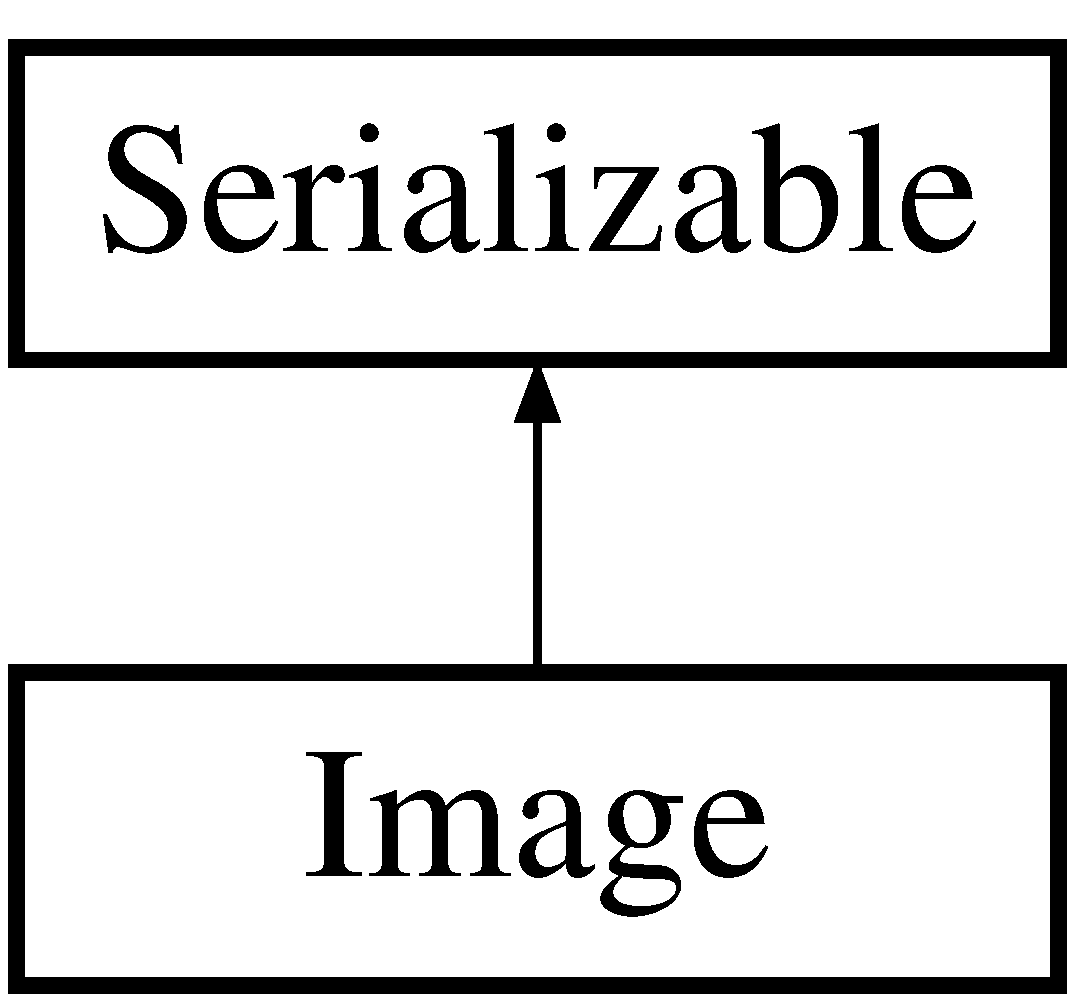
\includegraphics[height=2.000000cm]{classImage}
\end{center}
\end{figure}
\subsection*{Public Member Functions}
\begin{DoxyCompactItemize}
\item 
\hypertarget{classImage_ad68ef9e688d436493c1ad4598d3a85a9}{\hyperlink{classImage_ad68ef9e688d436493c1ad4598d3a85a9}{Image} (Buffered\-Image buf)}\label{classImage_ad68ef9e688d436493c1ad4598d3a85a9}

\begin{DoxyCompactList}\small\item\em inicializa altura e largura \end{DoxyCompactList}\item 
\hypertarget{classImage_a49851ce62d807ed254a9fc218a14483f}{Buffered\-Image \hyperlink{classImage_a49851ce62d807ed254a9fc218a14483f}{get\-Image} ()}\label{classImage_a49851ce62d807ed254a9fc218a14483f}

\begin{DoxyCompactList}\small\item\em Retorna dados da imagem lida, a imagem inteira. \end{DoxyCompactList}\end{DoxyCompactItemize}


\subsection{Detailed Description}
Classe \hyperlink{classImage}{Image}. 

Chamada na classe \hyperlink{classCliente}{Cliente}, classe que carrega dados da imagem e é enviada para o servidor 

The documentation for this class was generated from the following file\-:\begin{DoxyCompactItemize}
\item 
Image.\-java\end{DoxyCompactItemize}

\hypertarget{interfaceServidor}{\section{Servidor Interface Reference}
\label{interfaceServidor}\index{Servidor@{Servidor}}
}


Classe de \hyperlink{interfaceServidor}{Servidor}.  


Inheritance diagram for Servidor\-:\begin{figure}[H]
\begin{center}
\leavevmode
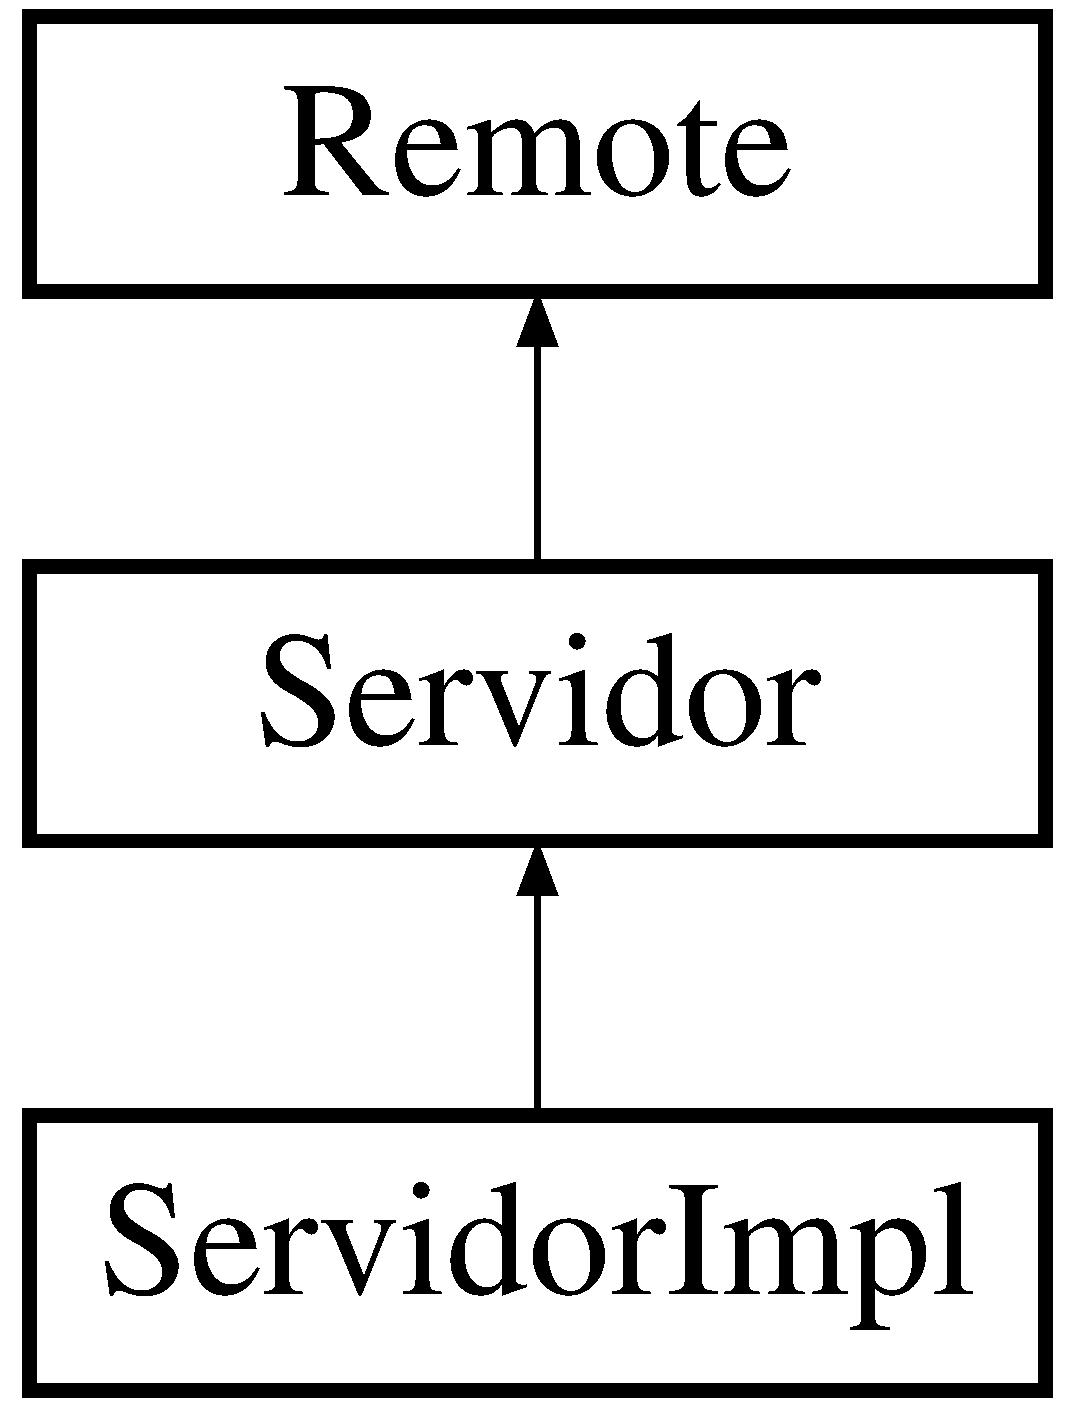
\includegraphics[height=3.000000cm]{interfaceServidor}
\end{center}
\end{figure}
\subsection*{Public Member Functions}
\begin{DoxyCompactItemize}
\item 
\hypertarget{interfaceServidor_a845e4c445fc700fa0a76a878dbe27ff5}{\hyperlink{classImage}{Image} {\bfseries Converter} (\hyperlink{classImage}{Image} c)  throws Remote\-Exception}\label{interfaceServidor_a845e4c445fc700fa0a76a878dbe27ff5}

\end{DoxyCompactItemize}


\subsection{Detailed Description}
Classe de \hyperlink{interfaceServidor}{Servidor}. 

Classe de interface \hyperlink{interfaceServidor}{Servidor} 

The documentation for this interface was generated from the following file\-:\begin{DoxyCompactItemize}
\item 
Servidor.\-java\end{DoxyCompactItemize}

\hypertarget{classServidorImpl}{\section{Servidor\-Impl Class Reference}
\label{classServidorImpl}\index{Servidor\-Impl@{Servidor\-Impl}}
}


Classe de \hyperlink{classServidorImpl}{Servidor\-Impl}.  


Inheritance diagram for Servidor\-Impl\-:\begin{figure}[H]
\begin{center}
\leavevmode
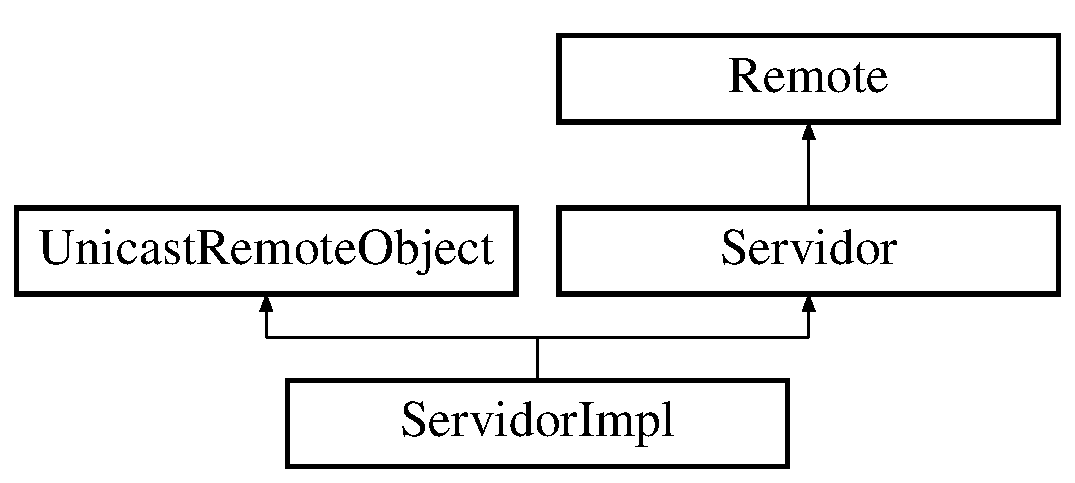
\includegraphics[height=3.000000cm]{classServidorImpl}
\end{center}
\end{figure}
\subsection*{Public Member Functions}
\begin{DoxyCompactItemize}
\item 
\hyperlink{classImage}{Image} \hyperlink{classServidorImpl_ab65c95968737a9f030e72c73838123a9}{Converter} (\hyperlink{classImage}{Image} c)  throws Remote\-Exception 
\begin{DoxyCompactList}\small\item\em Converte imagem para tons de cinza. \end{DoxyCompactList}\end{DoxyCompactItemize}


\subsection{Detailed Description}
Classe de \hyperlink{classServidorImpl}{Servidor\-Impl}. 

Possui método \hyperlink{classServidorImpl_ab65c95968737a9f030e72c73838123a9}{Converter()} 

\subsection{Member Function Documentation}
\hypertarget{classServidorImpl_ab65c95968737a9f030e72c73838123a9}{\index{Servidor\-Impl@{Servidor\-Impl}!Converter@{Converter}}
\index{Converter@{Converter}!ServidorImpl@{Servidor\-Impl}}
\subsubsection[{Converter}]{\setlength{\rightskip}{0pt plus 5cm}{\bf Image} Servidor\-Impl.\-Converter (
\begin{DoxyParamCaption}
\item[{{\bf Image}}]{c}
\end{DoxyParamCaption}
) throws Remote\-Exception\hspace{0.3cm}{\ttfamily [inline]}}}\label{classServidorImpl_ab65c95968737a9f030e72c73838123a9}


Converte imagem para tons de cinza. 

objeto buf

objeto recebe imagem de c.\-get\-Image

Conversão para tom de cinza

cria novas cor (vermelho, azul, verde) dos pixels da imagem e converte para tom de cinza cada pixel com novo inteiro gray, recebendo (red+green+blue)/3

Nova imagem

retorna nova imagem formada em tom de cinza

Implements \hyperlink{interfaceServidor}{Servidor}.



The documentation for this class was generated from the following file\-:\begin{DoxyCompactItemize}
\item 
Servidor\-Impl.\-java\end{DoxyCompactItemize}

\hypertarget{classServidorPrincipal}{\section{Servidor\-Principal Class Reference}
\label{classServidorPrincipal}\index{Servidor\-Principal@{Servidor\-Principal}}
}


Classe de \hyperlink{classServidorPrincipal}{Servidor\-Principal}.  


\subsection*{Static Public Member Functions}
\begin{DoxyCompactItemize}
\item 
\hypertarget{classServidorPrincipal_a311e49afdab7d66fa7ca73bb11dfb8b3}{static void {\bfseries main} (String\mbox{[}$\,$\mbox{]} args)}\label{classServidorPrincipal_a311e49afdab7d66fa7ca73bb11dfb8b3}

\end{DoxyCompactItemize}


\subsection{Detailed Description}
Classe de \hyperlink{classServidorPrincipal}{Servidor\-Principal}. 

Estabelece U\-R\-L, conexão 

The documentation for this class was generated from the following file\-:\begin{DoxyCompactItemize}
\item 
Servidor\-Principal.\-java\end{DoxyCompactItemize}

%--- End generated contents ---

% Index
\newpage
\phantomsection
\addcontentsline{toc}{chapter}{Index}
\printindex

\end{document}
